\documentclass[14pt]{extreport}
\usepackage{cmap}
\usepackage[utf8]{inputenc}
\usepackage[english,ukrainian]{babel}
\usepackage{graphicx}
\usepackage{geometry}
\usepackage{listings}
\usepackage{amsmath}
\usepackage{float}
\geometry{
	a4paper,
	left=20mm,
	right=20mm,
	top=20mm,
	bottom=20mm
}
\lstset{
	language=bash,
	tabsize=4,
	breaklines,
	keepspaces,
	showstringspaces=false,
}
\graphicspath{ {./pictures} }
\setlength{\parindent}{4em}

\newcommand\subject{Кросплатформне програмування}
\newcommand\lecturer{доцент кафедри ПЗ\\Дяконюк Л.М.}
\newcommand\teacher{ст. викл. кафедри ПЗ\\Шкраб Р.Р.}
\newcommand\mygroup{ПЗ-32}
\newcommand\lab{2}
\newcommand\theme{Робота з класами. Наслідування,
	поліморфізм. Створення класу-обгортки для
	колекції екземплярів. Сортування та пошук
}
\newcommand\purpose{Навчитися працювати з класами. Наслідування,
	поліморфізм. Створення класу-обгортки для
	колекції екземплярів. Сортування та пошук}

\begin{document}
\begin{normalsize}
	\begin{titlepage}
		\thispagestyle{empty}
		\begin{center}
			\textbf{МІНІСТЕРСТВО ОСВІТИ І НАУКИ УКРАЇНИ\\
				НАЦІОНАЛЬНИЙ УНІВЕРСИТЕТ "ЛЬВІВСЬКА ПОЛІТЕХНІКА"}
		\end{center}
		\begin{flushright}
			Інститут \textbf{КНІТ}\\
			Кафедра \textbf{ПЗ}
		\end{flushright}
		\vspace{160pt}
		\begin{center}
			\textbf{ЗВІТ}\\
			\vspace{10pt}
			До лабораторної роботи № \lab\\
			\textbf{На тему}: “\textit{\theme}”\\
			\textbf{З дисципліни}: “\subject”
		\end{center}
		\vspace{40pt}
		\begin{flushright}
			
			\textbf{Лектор}:\\
			\lecturer\\
			\vspace{10pt}
			\textbf{Виконав}:\\
			
			студент групи \mygroup\\
			Коваленко Д.М.\\
			\vspace{10pt}
			\textbf{Прийняв}:\\
			
			\teacher\\
			
			\vspace{28pt}
			«\rule{1cm}{0.15mm}» \rule{1.5cm}{0.15mm} 2023 р.\\
			$\sum$ = \rule{1cm}{0.15mm}……………\\
			
		\end{flushright}
		\vspace{\fill}
		\begin{center}
			\textbf{Львів — 2023}
		\end{center}
	\end{titlepage}
		
	\begin{description}
		\item[Тема.] \theme.
		\item[Мета.] \purpose.
	\end{description}
	
	\section*{Теоретичні відомості}
	\begin{itemize}
		\item У Java класи використовуються для опису об’єктів або сутностей, які мають специфічні характеристики і поведінку. Клас оголошується за допомогою ключового слова class.
		\item Java має вбудовані примітивні типи даних, такі як int, double, boolean, і т. д. Примітивні типи представляють базові значення і використовуються для зберігання даних.
		\item Утиліта Scanner використовується для зчитування даних з консолі. Ви можете використовувати її методи, такі як nextInt(), nextDouble(), nextLine(), тощо, для зчитування різних типів даних з консолі.
		\item Для роботи з довгими числами у Java використовується клас BigInteger з пакету java.math. BigInteger дозволяє виконувати операції з дуже великими цілими числами, які не вміщуються в примітивні типи.
	\end{itemize}

	\section*{Лабораторне завдання}
	Потрібно створити програму, яка обчислює суму ряду у вигляді звичайного нескоротного дробу для різних значень n. При значеннях параметра n, більших за 15 використовувати класи, призначені для роботи з довгими числами. 
	
	\section*{Хід роботи}

	\textbf{\textit{Main.java}}
	\begin{lstlisting}
import java.util.ArrayList;
import java.util.Comparator;
import java.util.List;
class House {
	private String name;
	private int distanceToSchool;
	private int distanceToPark;
	
	public House(String name, int distanceToSchool, int distanceToPark) {
		this.name = name;
		this.distanceToSchool = distanceToSchool;
		this.distanceToPark = distanceToPark;
	}
	
	public String getName() {
		return name;
	}
	
	public int getDistanceToSchool() {
		return distanceToSchool;
	}
	
	public int getDistanceToPark() {
		return distanceToPark;
	}
	
	@Override
	public String toString() {
		return "Housing{" +
			"name='" + name + '\'' +
			", distanceToSchool=" + distanceToSchool +
			", distanceToPark=" + distanceToPark +
			'}';
	}
}

class HousingManager {
	List<House> houses;
	
	HousingManager(List<House> houses) {
		this.houses = houses;
	}
	
	static class sortByDistanceToSchoolAsc implements Comparator<House> {
		@Override
		public int compare(House h1, House h2) {
			return Integer.compare(h1.getDistanceToSchool(), h2.getDistanceToSchool());
		}
	}
	
	class sortByDistanceToParkAsc implements Comparator<House> {
		@Override
		public int compare(House h1, House h2) {
			return Integer.compare(h1.getDistanceToPark(), h2.getDistanceToPark());
		}
	}
	
	public static Comparator<House> sortByDistanceToSchoolDesc() {
		return new Comparator<House>() {
			@Override
			public int compare(House h2, House h1) {
				return Integer.compare(h1.getDistanceToSchool(), h2.getDistanceToSchool());
			}
		};
	}
	
	public static Comparator<House> sortByDistanceToParkDesc() {
		return (h2, h1) -> Integer.compare(h1.getDistanceToPark(), h2.getDistanceToPark());
	}
}

public class Main {
	public static void main(String[] args) {
		List<House> houseList = new ArrayList<>();
		houseList.add(new House("Apartment A", 2, 1));
		houseList.add(new House("Penthouse B", 1, 5));
		houseList.add(new House("Mansion C", 4, 3));
		HousingManager mgr = new HousingManager(houseList);
		
		// Sort by distance to school (ascending) using static inner class
		houseList.sort(new HousingManager.sortByDistanceToSchoolAsc());
		System.out.println("Sorted by distance to school (ascending):");
		System.out.println(houseList);
		
		// Sort by distance to park (ascending) using inner class
		houseList.sort(mgr.new sortByDistanceToParkAsc());
		System.out.println("\nSorted by distance to park (ascending):");
		System.out.println(houseList);
		
		// Sort by distance to school (descending) using anonymous inner class
		houseList.sort(HousingManager.sortByDistanceToSchoolDesc());
		System.out.println("\nSorted by distance to school (descending):");
		System.out.println(houseList);
		
		// Sort by distance to park (descending) using lambda expressions
		houseList.sort(HousingManager.sortByDistanceToParkDesc());
		System.out.println("\nSorted by distance to park (descending):");
		System.out.println(houseList);
	}
}
		

	\end{lstlisting}	
	
	\begin{figure}[H]
		\centering
		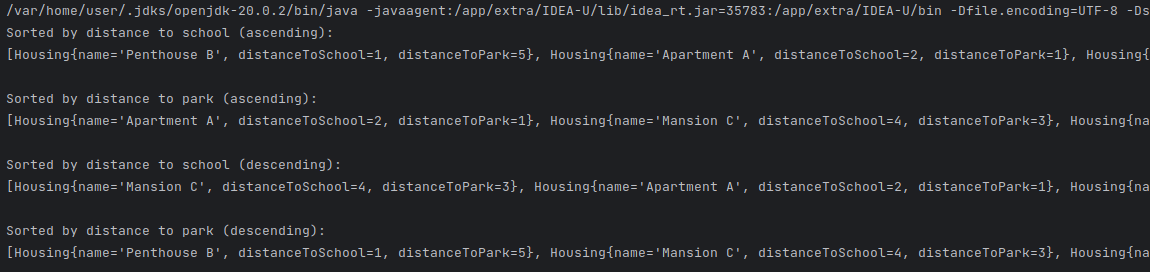
\includegraphics[scale=0.4]{1}
		\caption{Робота програми}
	\end{figure}

	\section*{Висновок}
	Під час виконання лабораторної роботи я працював з класами. Реалізував наслідування, поліморфізм. Створив клас-обгортки для
	колекції екземплярів.
	 
\end{normalsize}
\end{document}
